\chapter{Solution}
\label{chap:solution}

With a proper understanding of the Fenix Framework, this chapter
describes the solution proposed to solve the problem of relieving
programmers of the effort of programming Long Lived
Transactions. Section~\ref{sec:challenges} describes the challenges
faced when implementing Long Lived
Transactions. Section~\ref{sec:arch} describes the architecture of the
proposed solution, with the rationales for each design
decision. Section~\ref{sec:impl} describes how the proposed
architecture was implemented on top of the Fenix Framework using the
JVSTM. Finally, Section~\ref{sec:validation} shows that both the
architecture and implementation fullfil all the requirements, and
attempts to measure the effort required to use the implementation.

\section{Challenges}
\label{sec:challenges}

In Section~\ref{sec:difficult} I presented several approaches for
implementing Long Lived Transactions using the already existing
mechanisms. Two of those approaches required the programmer to rework
his code to support LLTs (keeping a parallel representation of the
domain and changing the domain model), which does not fit in the
requirements for this solution.

The only approach that did not require the programmer to modify his
domain code was keeping the database transaction open during the
multiple steps of the LLT. The reason this approach was not desirable
is that most DBMSs are not prepared to handle transactions open for
long periods of time.

A naive approach when implementing LLTs on top of the JVSTM could
simply be running each step on the context of a regular transaction,
suspending it in between steps, only committing it in the end of the
LLT. This approach presents several similarities with the approach
presented above, including some of the limitations:

\begin{itemize}

\item As the data is kept in transient memory, not only would LLTs not
  survive system restarts, but the memory usage of the system would
  also increase rather quickly.

\item As JVSTM transactions are not designed to be shared across
  multiple threads, supporting multiple concurrent users would
  require the usage of Parallel Nesting
  \cite{NunoMiguelLourencoDiegues2012}.

\end{itemize}

Despite this limitation, this approach is a step in the right
direction. With a few modifications, it is possible to overcome the
limitations and obtain a fully functional solution. To do so, there
are some challenges that need to be overcome:

\begin{itemize}

\item How is information persistently carried between the various
  steps of the transaction?

\item How to use a unique representation for every possible value any
  domain slot can take?

\item How to ensure that multiple users can concurrently access a Long
  Lived Transaction?

\end{itemize}

Throughout the rest of this chapter I will present solutions for these
challenges and create a solution that fulfils all the requirements.

\section{Architecture}
\label{sec:arch}

The main goal of this work is to relieve programmers of the burden of
dealing with Long Lived Transactions, making the effort needed to
program an LLT similar to the effort of programming a regular
transaction.

So, what does the single interaction scenario has that makes it so
easy to program? It has a single transactional context that spans the
whole operation (provided by the STM transaction). In the multiple
interaction scenario the system transaction was shorter than the
business transaction, so in each step the context was lost.

Looking at the information that is kept during the lifespan of a
regular transaction, we can identify three major pieces:

\begin{itemize}
\item The version in which the transaction is running. This version
  number corresponds to the logical point in time at which the
  transaction occurred (i.e. its serialization point).
\item A list of all the items written throughout the transaction (and
  the respective written values). This is the critical piece, as it
  contains the updated data that will be written to the global context
  on transaction's commit.
\item A list of all elements read throughout the transaction. This
  piece of information is critical to ensure the correctness of the
  operation, as the outcome of the transaction may depend on the
  values of all the read data.
\end{itemize}

These pieces are crucial to ensure the correct operation of an
STM-based transactional system. STM libraries provide them for regular
(short-lived) transactions. The solution presented below aims to
provide them for Long Lived Transactions, using the short-lived
transactions as its building blocks.

Short lived transactions keep all the necessary information in
transient transaction-local storage (typically in memory), until the
time they commit, merging the write set with the global context. With
Long Lived Transactions, merging this write set in each step is not
possible. 

Recall the Course creation example. Consider that in the first step a
Course is created with only a name and the department it is associated
to. Merging the Write Set for this step with the global context would
leave the system in an inconsistent state in which the departement is
associated to an unfinished course, as this transitory state would be
visible to the outside world.

There needs to be a way to persistently store the Write Set of each
step, outside the global context so that the changes are not visible
to the outside world. Only upon committing the Long Lived Transaction
these changes would be merged to the global context, meaning that the
writes performed by each step are effectively delayed until the end of
the transaction. Note that for correctness purposes, the Read Set of
the transaction must also be collected, so that at commit time both
Read Set and Write Set can be replicated, taking advantage of the
already existing JVSTM support.

As the main feature of the Fenix Framework is providing mechanisms to
transactionally manipulate and persist Domain Objects, perhaps it
would be a good approach to use regular Domain Objects to store the
required information.

\subsection{Data Structures}

\begin{figure}
\centering
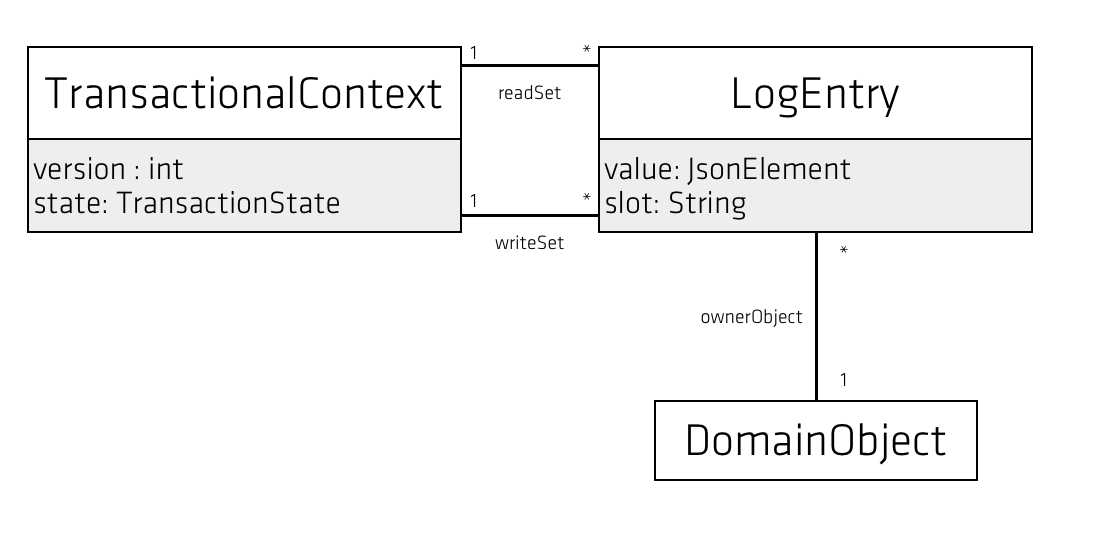
\includegraphics[width=0.8\linewidth]{tx-context}
\caption{Transactional Context's Domain Model}
\label{fig:transactionalContext}
\end{figure}

Consider the domain model presented in
Figure~\ref{fig:transactionalContext} that represents the reification
of the necessary data necessary for a transaction. A
\texttt{TransactionalContext} is the centerpiece of the domain, it
represents a Long Lived Transaction, holding together the entire state
of the transaction. By keeping the state of the LLT in regular domain
objects, we are ensuring that it is stored persistently (or at least
as persistent as the rest of the application) as well as
transactionally safe. Updates to the context are performed using a
regular transaction, allowing for multiple users to concurrently run
LLT steps (which will simply perform reads and writes to the context).

In this model, the \texttt{TransactionalContext} keeps the state of
the transaction (whether it is started, committed, aborted or in
conflict) and the version marker (corresponding to the ``current''
version when the first step of the transaction executed).

A context has two associated sets of \texttt{LogEntries}, one for the
Read Set and one for the Write Set. A \texttt{LogEntry} represents one
read or written slot throughout the transaction, by keeping a
reference to the object, slot name, as well as the value that was
written (note that the value is only kept if the LogEntry belongs to
the Write Set).

Once again recall the Course creation example, in which a Long Lived
Transaction is used to perform a multi-step creation of a new Course
for a given Department. To perform such operation, a new
\texttt{TransactionalContext} is created, initially empty
(Figure~\ref{fig:course-logEntries}a), with an undefined version.

\begin{figure}
\centering
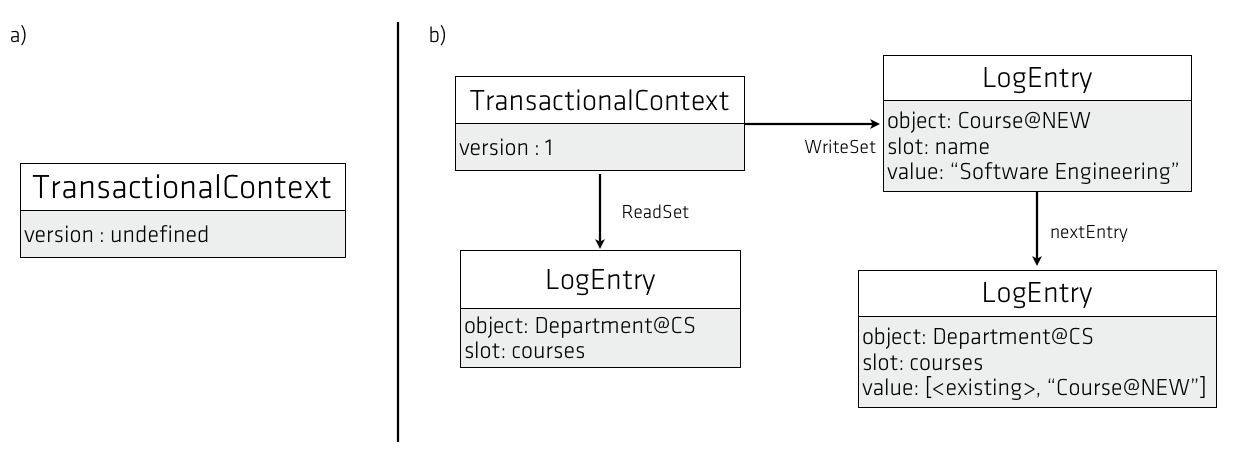
\includegraphics[width=1\linewidth]{log-entries}
\caption{Transactional Context instances in a Course creation transaction}
\label{fig:course-logEntries}
\end{figure}

In the first step, a new Course named ``Software Engineering'' is
created, and it is added to the CS department. As this step performed
a single read and two writes, three \texttt{LogEntries} are created: 
\begin{inparaenum}[\itshape a\upshape)]
\item In the Read Set representing the reading of the department's
  Course list
\item In the Write Set representing the updaded Course list for the CS
  department
\item In the Write Set representing the name slot for the newly
  created course.
\end{inparaenum}
Note that as this step was the first, the version of the
\texttt{TransactionalContext} is now defined as the ``current''
version. Figure~\ref{fig:course-logEntries}b shows the contents of the
context after the execution of the first step.

\subsection{Transaction Isolation}

Having the necessary data structures laid out is crucial for a proper
implementation of Long Lived Transactions, but it is just the
beginning. Whereas these structures are agnostic to the specific
backend, the backend must be able to recognise when a transaction is
executing within the context of a Long Lived Transaction, so that
reads and writes are isolated from the global context (otherwise the
whole world could see the intermediate values).

In the Fenix Framework, transactions are bound to a specific thread,
allowing for multi-threaded applications to execute multiple
concurrent transactions, each one in its own thread. As such, to run a
transaction in the context of a Long Lived Transaction, one must first
bind the context to the current thread. This way, when beginning a new
Transaction, the backend will check for the presence of a
\texttt{TransactionContext}, to determine whether to start a regular
transaction or a LLT step. Listing~\ref{list:longTxBind} shows the
programmer API for binding a \texttt{TransactionalContext} to a given
thread. This way, the programmer is free to run any piece of
transactional context as a step of a Long Lived Transaction.

\begin{lstlisting}[caption={Example of TransactionalContext usage},
  label={list:longTxBind},float]
public void runStep(TransactionalContext context) {
  try {
    // IllegalStateException if already within a context
    LongTransaction.setContextForThread(context);
    transactionalOperation();
  } finally {
    LongTransaction.removeContextFromThread();
  }
}

@Atomic
public void transactionalOperation() {
  (...)
}
\end{lstlisting}

Transactions occurring within the context of a Long Lived Transaction
must be aware of that fact, as this means that the semantics of domain
getters and setters is changed.

When reading the value of a slot within a
\texttt{TransactionalContext}, it is the responsibility of the backend
to check whether the slot is in the Write Set of transaction (so that
written values can be later read) and if it is not, read the value of
the slot in the correct version (the version recorded in the
context). Slot reads are recorded as a \texttt{LogEntry} in the Read
Set.

When writing the value of a slot, the written value is stored as a
\texttt{LogEntry} in the Write Set, so that it can later be retrieved
by read operations and used to update the state of other domain
objects when committing the transaction.

Backends will typically intercept reads and writes to the domain, and
use their regular methods for accessing the underlying transactional
context. As such, in the end of a step, only slots belonging to the
\texttt{TransactionalContext} and its \texttt{LogEntries} are written
to persistent support.

\subsection{Committing the Long Lived Transaction}

So far we have seen what data is stored in a
\texttt{TransactionalContext} and how it is populated. Now we shall
look at what happens when the Long Lived Transaction finishes, and the
context is committed.

Just like in a regular transaction, a Long Lived Transaction must be
atomic and consistent, meaning that its effects must appear to have
occurred at a single well-defined point in time. To accomplish this,
all elements of the Read Set must be validated to be in the same
version, thus ensuring that all writes were performed based on fresh
data (more details on how this is accomplished in
Section~\ref{sec:jvstm-commit}). If the validation step is successful,
all the written data must be merged into the global context, by
iterating over all \texttt{LogEntries} in the Write Set, and writing
the recorded value to the correct slot.

To ensure the correctness of the commit operation, both validation and
merge are performed within a regular transaction, in a
backend-specific manner (as only the backend knows how to write to an
arbitrary slot and to check if the read value is still valid). Any
conflicts on this operation, such as multiple concurrent commit
operations, or writes to validated slots will cause the commit
transaction itself to abort and restart.

Programmers can also manually rollback the Long Lived Transaction. In
this situation, all the information stored in the corresponding
\texttt{TransactionalContext} is deleted. As the Reads and Writes
performed by the transaction are stored exclusively in the context, no
further action is required.

\section{Implementation}
\label{sec:impl}


The previous section described a solution to ease the development of
Long Lived Transaction. This section describes how that solution was
implemented on the Fenix Framework, using the JVSTM as the
transactional support provider.

The implementation is divided in two parts:

\begin{enumerate}

\item The {\bf long-tx-api} module, which contains the domain
  specification of the \texttt{TransactionalContext} and
  \texttt{LogEntries}, as well as the API available to the programmer.

\item A {\bf JVSTM-based} implementation of Long Lived Transactions.
\end{enumerate}

The goal of this division is twofold: to allow alternative
implementations on top of non-JVSTM backends, and to hide internal
implementation details from the programmer (who should not depend on
backend code).

\subsection{API}

The {\bf long-tx-api} module is pretty straightforward. It contains
the domain definition described in
Figure~\ref{fig:transactionalContext}, The domain is public API, so
that Long Lived Transactions can be associated with any
programmer-defined object (e.g., to a user, to a group, a process
etc). This design decision allows for a simple solution, as
cross-cutting concerns such as security and sharing are abstract, and
also gives the programmer more flexibility.

It is the programmer's responsibility to instantiate a new
TransactionalContext every time a new Long Lived Transaction is to be
started. With the context in hand, the programmer simply needs to bind
it to the thread running the step. Listing~\ref{list:longTxBind} shows
the code necessary to bind the context to a thread.

Using only this simple API, the programmer is able to easily code
features that benefit from Long Lived Transactions with little effort.

\subsection{JVSTM implementation}

In the proposed architecture, several features are required to be
provided by the backend:

\begin{itemize}

\item {\bf Context Detection} The backend detects the presence of a
  \texttt{TransactionalContext} in the current thread, and begins a
  context-aware transaction.

\item {\bf Intercepting reads/writes} Ensure that reads and writes
  performed in LLT steps are not performed to the global context.

\item {\bf Context commit} Once the Long Lived Transaction is
  finished, merge its changes with the global context.

\end{itemize}

\subsubsection{Context Detection}

When beginning a transaction in \texttt{jvstm-common}, the backend
checks for the presence of a \texttt{TransactionalContext} bound to
the current thread, and if one is present, the following happens:

\begin{enumerate}

\item A regular transaction is started. This transaction will be used
  to access the context and previous versions of VBoxes (for when a
  read is made and the context cannot not provide a value).

\item A nested \texttt{LLTStepTransaction} is started. This will be the
  active transaction, and route reads and writes to the corresponding
  \texttt{TransactionalContext}.

\item In case this is the first step of the LLT, it is necessary to
  define its version. To ensure that every other step of the LLT has
  the same view of the world as this one, mark the LLT's version as
  the version of the current transaction.

\end{enumerate}

\begin{lstlisting}[caption={Beginning a new Long Lived Transaction
    step}, float]
if (LongTransactionSupport.isInsideContext()) {
  TransactionalContext context = 
      LongTransactionSupport.getContextForThread();

  // Begin a new Top Level Write-Transaction
  JvstmInFenixTransaction underlying =
      Transaction.begin(false);

  LLTStepTransaction longTx = 
      new LLTStepTransaction (context, underlying);

  longTx.start();

  transactions.set(new JVSTMTransaction(longTx));
}

(...)

// In the beginning of the new transaction
if (context.getVersion() == null) {
  context.setVersion(Transaction.current().getNumber());
}
\end{lstlisting}

The main reason to use a Nested transaction is to allow portability
across concrete persistence implementations, as the
\texttt{LLTStepTransaction} will be agnostic to the specific
underlying transaction (provided it fulfils the required API). A
\texttt{LLTStepTransaction} holds a reference to the
\texttt{TransactionalContext} backing it, so that it can be used to
aid in reading and writing.

\subsubsection{Intercepting Reads and Writes}

As in the JVSTM backend each domain object slot is backed by a VBox,
intercepting reads and writes to slots can be easily done. The
implementation of the get/set methods in a VBox simply delegates the
read/write to the current transaction.

As such, the \texttt{LLTStepTransaction} was introduced. Its goal is
to intercept the reading and writing of boxes, ensuring that such
reads and writes are both isolated from the outside world and
collected into the \texttt{TransactionalContext}.

Just like regular transaction, writing a VBox will simply keep the
written value in the transaction's Write Set. This Write Set will be
processed when committing the step. 

\begin{lstlisting}[caption={Reading a VBox within a Context},float]
public <T> T getBoxValue(VBox<T> vbox) {
  // Check the local Write Set
  T result = getLocalValue(vbox);
  if (result == null) {
    if (vbox.getOwnerObject().
          getClass().isAnnotationPresent(NoLogEntries.class)) {
      // For classes annotated with @NoLogEntries
      // check the parent transaction in the current version
      return parent.getBoxValue(vbox);
    }

    // Check the TransactionalContext
    result = lookupBoxValueInContext(vbox);
    if (result == null) {
      // Read from the parent
      result = parent.getPreviousBoxValue(vbox, version);
      bodiesRead.put(vbox, null);
    }
  }
  return result == NULL_VALUE ? null : result;
}

private <T> T lookupBoxValueInContext(VBox<T> vbox) {
  LogEntry writeSetEntry = context.getWriteSet();
  while (writeSetEntry != null) {
    if (writeSetEntry.getDomainObject().
                             equals(vbox.getOwnerObject()) &&
        writeSetEntry.getSlotName().
                             equals(vbox.getSlotName())) {
      String contents = writeSetEntry.getContents();
      return vbox.getOwnerObject().
                         getValueFromJSON(vbox.getSlotName(),
                                                       contents);
    }
    writeSetEntry = writeSetEntry.getNextEntry();
  }
  return null;
}


\end{lstlisting}

When reading a VBox within a \texttt{LLTStepTransaction}, the following
steps are executed:

\begin{enumerate}

\item If the VBox was previously written in this step, return the
  written value. This is accomplished by looking up the value in the
  step's own transient Write Set.

\item In case the VBox being read belongs to either a
  \texttt{TransactionalContext} or a \texttt{LogEntry}, the read is
  delegated to the parent transaction in the current version (so that
  always the latest version is read). Such reads will typically be
  nested within reads of other boxes, when the context's Write Set is
  being searched.

\item If the VBox was written in a previous step of the Long Lived
  Transaction, return the previously written value, obtained from a
  \texttt{LogEntry} in the Write Set of the LLT.

\item Else, delegate the read to the underlying transaction, in the
  same version as the context, and add the VBox to the current
  transaction's Read Set.

\end{enumerate}

As domain slots can hold virtually any value, it is not possible to
store the value directly in a single statically typed Fenix Framework
slot. To solve this issue, the values are stored in JSON format, in a
single slot on the \texttt{LogEntry} class. Recall from
Section~\ref{sec:json} that the Fenix Framework provides native
support for converting any ValueType to/from JSON. With a little help
from the backend-specific Code Generation step, domain objects can now
be asked to convert the value of a given slot to/from JSON, making it
possible for Long Lived Transactions to get a JSON value from any
VBox.

When the transaction finishes, the \texttt{LLTStepTransaction} has in
its Read and Write Sets the actual VBoxes that were read/written
during the transaction. Recall that in each step the Read Set and
Write Set of the step must contain only the changes to the context
that reflect what has been read and written. As such, when committing
the step, the Read Set and Write Set are processed in the following
manner:

\begin{lstlisting}[caption={Algorithm for committing a Long Lived
    Transaction's step}, float]
protected void tryCommit() {
  // Go through the ReadSet and the WriteSet
  // No consistency validations are performed here, as the 
  // purpose of this transaction is to manipulate the contents
  // of the read/write set.
  Map<VBox, Object> originalWriteSet = 
                new HashMap<VBox, Object>(boxesWritten);
  Set<VBox> originalReadSet = new HashSet(bodiesRead.keySet());

  // Clear read/write-set, will be populated with LogEntries
  boxesWritten.clear();
  bodiesRead.clear();

  for (Entry<VBox, Object> entry : originalWriteSet.entrySet()) 
  {
    VBox<?> vbox = (VBox<?>) entry.getKey();

    JVSTMDomainObject owner = vbox.getOwnerObject();

    // Get the JSON value with a little help
    // from Generated Code
    String json = 
          owner.getJSONStringForSlot(vbox.getSlotName(), 
                                     entry.getValue());

    // Create or update the LogEntry
    context.addWriteSetEntry(owner, vbox.getSlotName(), json);
  }

  for (VBox vbox : originalReadSet) {
    // Create a new LogEntry if this slot wasn't
    // read in a previous step
    context.addReadSetEntry(vbox.getOwnerObject(), 
                            vbox.getSlotName());
  }

  // Add the new read/written boxes to the parent transaction,
  // which will ensure the LogEntries are properly committed
  super.tryCommit();
}
\end{lstlisting}

\begin{enumerate}

\item The original Read and Write Sets are backed up and cleared.

\item For each item in the original Write Set, the written value is
  converted to JSON and it is added to the
  \texttt{TransactionalContext}. As this operation is still running
  within the context of the transaction, the changes are added to the
  real Write Set transparently.

\item The same is done to the Read Set.

\item The new Read and Write Sets are merged with the parent
  transaction, and the nested transaction is committed.

\end{enumerate}

Once the nested transaction is committed, the parent
(backend-specific) transaction will ensure that the updated
\texttt{TransactionalContext} is stored in persistent support. Note
that the only objects written will be the ones representing the
context and its \texttt{LogEntries}.

\subsubsection{Finishing the Long Lived Transaction}
\label{sec:jvstm-commit}

Once all steps of the Long Lived Transaction are finished, the
transaction must be committed, ensuring that the changes performed in
it are visible to the outside world. Much of this process is heavily
dependent on the backend as it involves direct access to the
underlying data structures.

The commit process of a Long Lived Transaction occurs within a regular
transaction. In this process, the data collected throughout the
multiple steps is validated and replayed. Once this transaction
commits, all written data will be merged with the global context.

The first step in committing the context is verifying whether all the
read data is still valid. As every slot is mapped in a JVSTM VBox, all
the boxes corresponding to the read slots must be verified. The
process iterates over all read slots, locating the VBox that
represents the slot. It then reads the VBox, so that it is added to
the Read Set of the current transaction. Then, the latest version of
the VBox is compared to context's version, thus ensuring that the read
value was the latest. If the box's current version if posterior to the
read version, the Long Lived Transaction is aborted.

There is a critical subtlety in this verification
process. Modifications to the VBox's underlying data structures are
performed only at commit time, inside a commit lock. As the
verification process is not run within the commit lock, it is possible
for another transaction to concurrently update a VBox after the
validation. Preventing incorrect behaviour is quite simple: Just read
the box. By doing this, the box will be validated when the transaction
commits, ensuring that the verification was correct (i.e. the version
read during the verification is still valid).

Consider the following scenario: VBox A was read in a Long Lived
Transaction in version 1 and not changed afterwards. When the Long
Lived Transaction commits (in a transaction X), A will be validated,
its current version (1) compared to the version of the transaction
(1). It passes the test and validation succeeds, proceeding with the
commit. Concurrently (after the validation, before X commits), another
transaction writes to A and commits, increasing its version to (X+1). When
X attempts to commit, its read set (which mirrors the Read Set of the
Long Lived Transaction) is validated. As A was concurrently written, X
will be restarted, and the version verification will fail, marking the
Long Lived Transaction as conflicting.

Once the Read Set of the Long Lived Transaction is validated, the
Write Set must be merged into the global context. This process
iterates over the written slots, and for each slot: (1) Locates the
VBox representing it, (2) Converts the JSON value to the concrete value,
and (c) Writes the value to the VBox.

After the merge process is finished, the committing transaction has a
full mirror of the LLT's Read and Write Sets, and once it commits,
every change in the Write Set is available to the outside world.

\begin{lstlisting}[caption={Implementation of the Long Lived
    Transaction commit operation},float]
void commitContext(TransactionalContext context) {
  // Don't do anything if nothing was written
  if (context.getWriteSet() != null) {
    if (!validateContext(context)) {
      throw new TransactionError();
    }
    mergeContext(context);
  }
}

boolean validateContext(TransactionalContext context) {
  int version = context.getVersion();
  LogEntry readSetEntry = context.getReadSet();
  while (readSetEntry != null) {
    JVSTMDomainObject owner = readSetEntry.getDomainObject();

    VBox box = owner.getBoxForSlot(readSetEntry.getSlotName());

    // Read the box to ensure it goes in the read set of 
    // the current transaction. This way, if a concurrent 
    // transaction writes to this box between this version
    // check and the commit of this transaction, it will
    // be restarted
    box.get();

    if (box.body.version > version) {
      // This means that the box was written after the LLT
      // started, meaning it has to be aborted.
      return false;
    }
    readSetEntry = readSetEntry.getNextEntry();
  }
  return true;
}

void mergeContext(TransactionalContext context) {
  LogEntry entry = context.getWriteSet();
  while (entry != null) {
    JVSTMDomainObject owner = entry.getDomainObject();
    VBox box = owner.getBoxForSlot(entry.getSlotName());
    box.put(owner.
                getValueFromJSON(writeSetEntry.getSlotName(), 
                                 writeSetEntry.getContents()));
    entry = entry.getNextEntry();
  }
}
\end{lstlisting}

\section{Validation}
\label{sec:validation}

This chapter proposed a solution that allows programmers to take
advantage of Long Lived Transactions with little effort and no code
modifications. I shall now validate the proposed solution, both in
terms of correctness and ease of use.

\subsection{Correctness}

One of the greatest challenges when implementing Long Lived Transactions
is ensuring that the solution provides the same correctness guarantees
as regular transactions. I will now demonstrate that the proposed
solution provides the same correctness guarantees as regular transactions.

Transactions in the JVSTM are ACI compliant (they provide Atomicity,
Consistency and Isolation), with an Opacity isolation level (refer to
Section~\ref{sec:opacity}). When integrated with the Fenix Framework,
transactions may also provide the Durability property, depending on
whether the concrete backend supports persistence.

The proposed solution also provides all the ACID properties for Long
Lived Transactions, as well as an Opacity isolation level.

\begin{itemize}

\item {\bf Atomicity} is provided as all the writes performed during
  the LLT are only written to the global context when the it commits,
  which is performed by a regular transaction.

\item {\bf Consistency} is provided in the same way as a regular
  transaction, by ensuring that every read is still valid at commit
  time.

\item {\bf Isolation} is provided as no data is ever written to the
  global context until the LLT is finished, and data reads are isolated.

\item {\bf Durability} is provided if the underlying backend supports
  data persistence.

\end{itemize}

Throughout the execution of the Long Lived Transaction, written data
is collected and stored inside the \texttt{TransactionalContext}. Once
the transaction is finished, written data is {\bf atomically} written
to the global context, using a regular transaction which simply reads
data from one domain object (the context) to be written in another
(the actual objects written during the transaction).

Long Lived Transactions are {\bf consistent}. Similarly to regular
transactions, a LLT only commits if all the data read during the
transaction is still valid at commit time. This is done by comparing
the version of the LLT against the version of every box in the Read
Set, just like a regular transaction would do.

{\bf Isolation} is perhaps the hardest property to demonstrate. When
performing a read operation within a Long Lived Transaction, the
system ensures that the returned value will be the one at the moment
the first step of the LLT executed (i.e. the value consistent with the
transaction's version), just like it happens with regular
transactions.  As for writes, similarly to what happens with regular
transactions, written values are kept in transaction-local storage
(i.e. in \texttt{LogEntries}) and as such, can only be accessed by the
transaction itself.


{\bf Durability} is an ``optional'' property, as not all JVSTM-based
backends provide persistent support. Those that do however, ensure
that the effects of Long Lived Transactions as durable, as it works as
if writes occurred in a single regular transaction (which already
provides the Durability property).

I have shown that Long Lived Transactions provide the same correctness
guarantees as regular transactions. There is, however, one key piece
missing. Correctness is only guaranteed provided that all the
information about reads and writes is collected throughout the
transaction, and is available at commit time.

Recall from the previous sections that in each step of the Long Lived
Transaction, every read and write operation is intercepted, and for
each operation a record is created. Such records are kept in
\texttt{LogEntries}, which in turn are writting using regular
transactions. As such, once the LLT is committing, it is able to read
all the recorded data, and use it for all the necessary verifications
and data updates.

\subsection{Ease of Use}

The primary goal of this work is to ease the development of Long Lived
Transactions, and as such, it is rather important to provide a simple
and concise API.

The proposed solution fares well in that regard, as it allows existing
code to be adapted to use Long Lived Transactions with no
modifications. It is possible to program the business logic of your
whole application using regular transactions, and with a simple
wrapper add Long Lived Transaction support.

Consider a Web Application wishing to share with its users the
benefits of Long Lived Transactions, by allowing each individual user
to keep a series of Long Operations. Support for this feature could be
added at an infrastructural level, by providing the user with a UI to
manage his Operations (creating, committing, enabling, etc). Creating
and committing the operation would imply simple domain object
manipulation (in particular creating and committing a
\texttt{TransactionalContext}).

Making every action performed by the user as a step of the Long Lived
Transaction would be a simple as keeping the context in session-local
storage, and binding it before every transaction start (using a Web
Filter or similar). With this architecture, it is possible to make
EVERY operation in the application part of a Long Lived Transaction,
without the need to change existing code, or changing the methodology
used to develop new functionalities.

